\hsection{The Objective Function}%
\label{sec:objectiveFunction}%
%
We now know the most important elements of input and output data for an optimization algorithm: the problem instances~\instance\ and candidate solutions~$\solspel\in\solutionSpace$, respectively.
But we do not just want to produce some output.
We do not just want to find \inQuotes{any} candidate solution.
We want to find the \inQuotes{good} ones.
For this, we need a measure rating the solution quality.%
%
\hsection{Definitions}%
%
\begin{definition}[Objective Function~\objf]%
\label{def:objectiveFunction}%
An \emph{objective function}~$\objf:\solutionSpace\mapsto\realNumbers$ numerically rates the quality of a candidate solution $\solspel\in\solutionSpace$ from the solution space~\solutionSpace.%
\end{definition}%
%
\begin{definition}[Objective Value~\obspel]%
\label{def:objectiveValue}%
An \emph{objective value}~$\obspel=\objfOf{\solspel}$ of the candidate solution~$\solspel\in\solutionSpace$ is the value that the objective function~\objf\ takes on for~\solspel.%
\end{definition}%
%
\begin{definition}[Minimization]%
\label{def:minimization}%
An objective function is subject to \emph{minimization} if smaller objective values indicate better solutions.%
\end{definition}%
%
\begin{definition}[Maximiation]%
\label{def:maximization}%
An objective function is subject to \emph{maximization} if larger objective values indicate better solutions.%
\end{definition}%
%
Without loss of generality, we assume that all objective functions are subject to \emph{minimization}.
In this case, a candidate solution~$\solspel_1\in\solutionSpace$ is better than another candidate solution~$\solspel_2\in\solutionSpace$ if and only if~$\objfOf{\solspel_1}<\objfOf{\solspel_2}$.
If~$\objfOf{\solspel_1}>\objfOf{\solspel_2}$, then~$\solspel_2$ would be better and for~$\objfOf{\solspel_1}=\objfOf{\solspel_2}$, there would be no benefit in choosing either solution over the other, at least from the perspective of the optimization criterion~\objf.
The minimization scenario fits to situations where \objf~represents a cost, a time requirement, or, in general, an amount of required resources.

In the \gls{TSP}, for example, a tour is better if it is shorter.
In the \gls{BPP}, a packing plan is better if it requires fewer bins.

Maximization problems, i.e., where the candidate solution with the higher objective value is better, are problems where the objective function represents profits, gains, or any other form of positive output or result of a scenario.
Maximization and minimization problems can be converted to each other by simply negating the objective function.
In other words, if \objf~is the objective function of a maximization problem, we can solve the minimization problem with objective~$-\objf$ and get the same result, and vice versa.%
%
\endhsection%
%
\hsection{A Programmer's Perspective}%
%
From the perspective of a programmer, the general concept of objective functions can be represented by the \codeil{class} given in \autoref{lst:Objective}.
The \codeil{evaluate} function of this class accepts one element~\codeil{x} from the solution space and returns a numerical value.
We can implement this function in any way we want, meaning that we can accommodate all types of solution spaces and optimization goals.%
%
\moptipyCode{moptipy/api/objective.py}{--labels book --args doc}{Objective}{A base class for objective functions.}%
%
\endhsection%
%
\hsection{Example: Job Shop Scheduling}%
\label{sec:jsspObjectiveFunction}%
%
What could be a suitable objective function for the \gls{JSSP}?
As stated in \autoref{sec:jsspExample}, our goal is to complete the production jobs as soon as possible.%
%
\begin{definition}[Makespan]%
\label{def:makespan}%
In manufacturing, the \emph{makespan} is the time difference between the start and finish of a sequence of jobs or tasks.%
\end{definition}%
%
Since we assume that all jobs begin at time index~0 in our Gantt charts, the makespan is the time when the last operation of the last job is finished.
Obviously, the smaller this value, the earlier we are done with all jobs, the better is the plan.
The makespan is therefore subject to minimization.
As illustrated in \autoref{fig:gantt_demo_with_makespan}, the makespan is the time index of the right-most edge of any of the machine rows/schedules in the Gantt chart.
In the figure, this happens to be the end time~230 of the last operation of job~0, executed on machine~4.

\begin{figure}%
\centering%
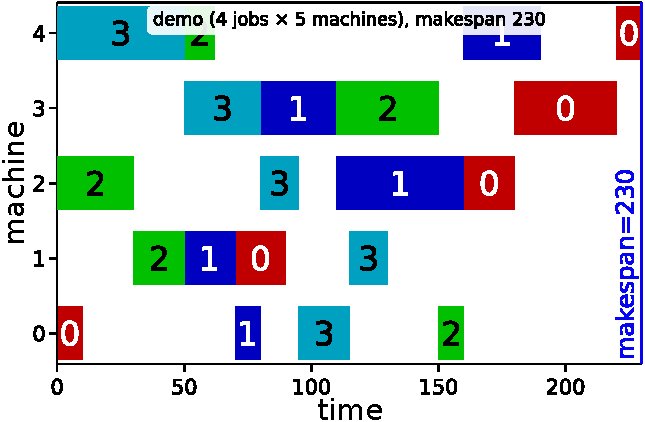
\includegraphics[width=0.55\linewidth]{\currentDir/gantt_demo_with_makespan.pdf}%
\caption{The makespan, i.e., the time when the last job is completed, for the example candidate solution illustrated in \autoref{fig:gantt_demo_without_makespan} for the \instStyle{demo} instance from \autoref{fig:jssp_demo_instance}.}%
\label{fig:gantt_demo_with_makespan}%
\end{figure}

Our objective function~\objf\ is thus equivalent to the makespan and subject to minimization.
Based on our candidate solution data structure \codeil{Gantt} developed \autoref{lst:jssp_gantt}, we can easily compute~\objf.
Remember that each instance of \codeil{Gantt} is basically a \numpyndarray\ with three dimensions.
The first dimension (accessed via the first index~\jsspMachineIndex) is the machine index.
The second dimension (accessed via the second index~$k$) lets us access the operations in the order in which they are carried out on that machine.
To compute the makespan, we need to only access the very last operation done on any machine.
For this, we can set second index to~$k=-1$, which, in Python, gives us the last element of a \codeil{list} or \numpyndarray.
Finally, in the third dimension (accessed via the third index~$l$), we store the job~ID (at~$l=0$), the start time (at~$l=1$), and the end time of the operation (at~$l=2$).
Obviously, we only need that last value, so we can set the third index to~$l=2$.
So the second and third index into a \codeil{Gantt} chart matrix are defined and we only need to compute the maximum value that we get for any of the possible values of first index.
In \autoref{lst:jssp_makespan}, we implement exactly this concept in the easiest possible way.
(For the Python aficionado: we apply the performance tricks from TODO.)

\moptipyCode{moptipy/examples/jssp/makespan.py}{--labels book --args doc,comments}{jssp_makespan}{An implementation of the \codeil{class Objective} \autoref{lst:Objective} to represent the makepan objective function for \glspl{JSSP}.}

With this objective function~\objf, subject to minimization, we have defined that a Gantt chart~$\solspel_1$ is better than another Gantt chart~$\solspel_2$ if and only if $\objfOf{\solspel_1}<\objfOf{\solspel_2}$.\footnote{under the assumption that both are feasible, of course}
\endhsection%
%
\hsection{Summary}%
%
The objective function~\objf\ is the third crucial component of optimization problems.
The instance data~\instance\ gives us the definition of a specific scenario as \emph{input}.
The solution space~\solutionSpace\ contains all the possible solutions and we will return at least one candidate solution~$\solspel\in\solutionSpace$ \emph{output} of our algorithm.
%
\ruleOfThumb{returnObjectiveValue}{For each solution~$\solspel\in\solutionSpace$ returned as output of an optimization algorithm, we should also return the corresponding objective value~$\obspel=\objfOf{\solspel}$.}%
%
\endhsection%
\endhsection%
%
